%/**********************************************************************/
%		第2章:CAMベースリアルタイム符号化テーブル最適化ハフマン符号化アーキテクチャ
%/**********************************************************************/
\chapter{CAMベーステーブルルックアップ符号化処理}
\label{lbl_chptr3}

本章では,マルチメディアデータを高圧縮に
処理することのできる,CAMベースのテーブルルックアップアーキテクチャを提案する.
提案アーキテクチャは,テーブルルックアップ処理を高速に行いつつ,
リアルタイムに圧縮に用いる符号化テーブルを最適化して圧縮効率の
向上を実現するものである.
また,提案アーキテクチャは本論文の研究目的である,
高性能CAMベース超並列SIMD型プロセッサにおける
高圧縮処理の基本となる技術となっている.

%マルチメディアデータの高圧縮処理のために,CAMを用いたマルチメディアデータ高圧縮
%処理のアーキテクチャを提案し,処理能力や他アーキテクチャとの性能評価について述べる.

本章の構成は以下の通りである.\ref{lbl_cp3}節において,提案アーキテクチャの実現目標を示し,
\ref{lbl_cp3_realtime_huffman}節にて,提案アーキテクチャのターゲットアルゴリズムである
ハフマン符号化について述べる.
\ref{lbl_cp3_real_opti_huffman}節では,提案アーキテクチャの構成について詳述し,
\ref{lbl_cp3_impl}節にて,FPGAへの実装結果について説明する.
\ref{lbl_cp3_jpeg_huffman}節では,ハフマン符号化が用いられているJPEGアプリケーションに提案アルゴリズムを
適用した場合の性能評価について言及し,
提案アーキテクチャをLSI化した際のハードウェアコストについて,
\ref{lbl_cp3_hrd_cst}節にて述べる.
%また,\label{lbl_cp3_hrd_mlt}節では,CAMのマルチプルマッチを利用した,提案アーキテクチャの応用例について述べ
最後に\ref{lbl_cp3_hrd_matome}節にて,本章のまとめとする.




%/**********************************************************************/
%		イントロの章
%/**********************************************************************/
\section{はじめに}
\label{lbl_cp3}

近年のマルチディア環境の急激な発展に伴い,
データのリアルタイムな高圧縮処理の重要性については
\ref{lbl_cp1_ashuku_tech}節及び\ref{lbl_cp1_ashuku}節にて述べた.
圧縮処理には大きく分けて,可逆圧縮 (Lossless compression)アルゴリズムと
非可逆圧縮 (Lossy compression)アルゴリズムがある.
可逆圧縮とはデータの欠落が全く起こらない圧縮方式のことであり,
復号によって圧縮前のデータを完全に再現可能とするアルゴリズムである.
この圧縮方法は圧縮率は大きくないものの,プログラムや文字データ等,データの欠損が
重大な損失を起こすコンテンツに使用される.
非可逆圧縮は,この逆でありデータの圧縮率が大きいものの,完全に前の状態には復元できない.
そのため,音声や画像のような多少のデータの欠落に対しても品質を大きく損なう恐れの無い
コンテンツに使用されることが多い.

本章では,代表的な可逆圧縮アルゴリズムであるハフマン符号化
%\cite{xx}
を圧縮アルゴリズムに
利用し,可逆圧縮と非可逆圧縮それぞれの長所を実現可能な
CAMをベースとしたリアルタイムに高圧縮処理が可能なアーキテクチャを提案する.



%/**********************************************************************/
%		動的にハフマン符号化テーブルを更新することのできるアルゴリズムを提案する章
%/**********************************************************************/
\section{ハフマン符号化}
\label{lbl_cp3_realtime_huffman}

ハフマン符号化は,データ圧縮技術の中でも,最も効率のよいロスレス圧縮技法の一つとして知られている\cite{hufmcm}.
このアルゴリズムは,圧縮対象のデータ (記号)に対して可変長の符号を割り当てるものであり,各データのうち生起確率の大きい,
すなわち頻繁に出現する記号には短いビット長の符号を割り当て,生起確率の小さい,稀にしか出現しない記号には
長いビット長の符号を割り当てる符号化方式である.
一般にこの割り当てはハフマン木と呼ばれる,各記号の生起確率に基づいた木を構築することで行われる.
各葉に対応する記号の生起確率 (及びそれらの和)を重みとして持たせ,
重みの大きい順に記号を組み合わせることでハフマン木を構築し,根から葉にたどることにより符号化を行う.
図 \ref{huffman_tree}にハフマン木の構築例を示す.ハフマン木の構築法及び符号の割り当ては以下の手順で行う.

\begin{enumerate}
\item 各記号の生起確率を求める.
\item 記号を生起確率の大きさ順に並べる.
\item 生起確率の小さいものから2つ選択し和を取る.この際枝の上から0,1を付加する.
\item 記号ごとに根から葉までたどることで対応する記号の符号化が完了する.
\end{enumerate}

この手順で処理を行うと,図 \ref{huffman_tree}中の\#で表している順番で木を構築することとなり,例えば記号Eの場合,``1110"のハフマン符号
を割り当てることができる.
図 \ref{huffman_tree}の場合には各記号がASCIIコードで表されているとすると,
「ABCDEFG」のデータは56 bit必要であるところを,24 bitで済むこととなる.
この結果,全体のデータ量を削減することができる.
以下にハフマン符号化の特徴をまとめる.

\begin{itemize}
	\item 可変長符号\\
			圧縮する記号それぞれに長さの異なる符号を割り当てる.
	\item データの一意性\\
			デコードデータの解釈が一通りである.
	\item 可逆圧縮 (ロスレス圧縮)\\
			符号化されたデータから圧縮前のデータを損失なく,完全に復元することが可能である.
\end{itemize}

ハフマン符号化は,圧縮処理を行う前に現れる記号列を基にして,はじめに符号化テーブルを作成し,
再び同様の記号列に対し作成した符号化テーブルを用いて圧縮を行う.
しかしながらこの方法では,圧縮を行うためにデータを2回スキャンする必要があるため,
オンラインでのリアルタイム圧縮は困難となる.
そこで,現在のハードウェアによるハフマン符号化の実装形態は,大きく分けて
静的ハフマン符号化 (Static Huffman Coding)\cite{hufmcm}と
動的 (適応型とも呼ぶ)ハフマン符号化 (Adaptive Huffman Coding)\cite{kundhc85}の
2通りに分かれている.以下では,それぞれの現状とその問題点について述べる.

% figure*
	\begin{figure*}[tbh]
	\centering
		\begin{center}
			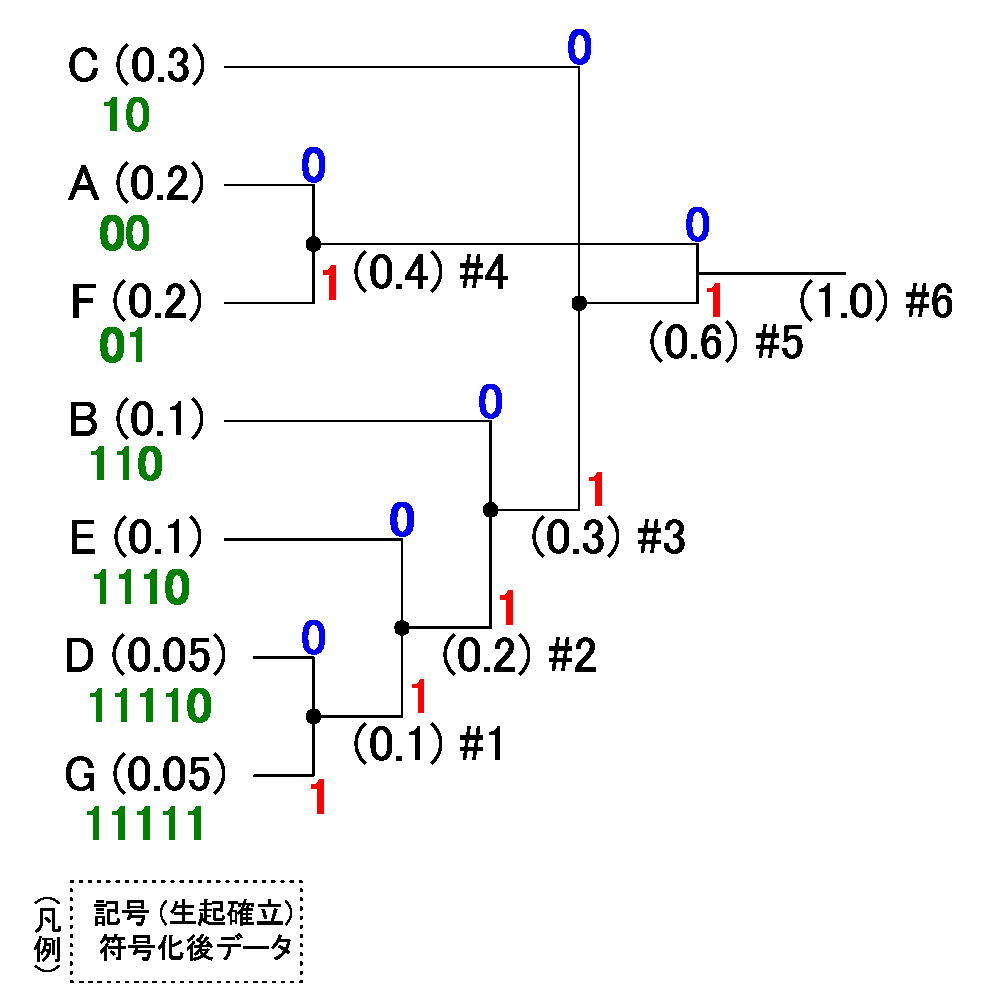
\includegraphics[width = 12cm,  height = 12cm,  keepaspectratio, clip]{./pics/huffman_tree.eps}
		\caption{ハフマン木構築例.}
		\label{huffman_tree}
		\end{center}
	\end{figure*}%	
%figure*

\subsection{静的ハフマン符号化方式 (Static Huffman Coding)}
\label{lbl_cp3_seiteki_huffman}
静的ハフマン符号化は最も広く実装されている形態である.
符号化をリアルタイムに実行するために,あらかじめ数多くのサンプルデータから,
データの出現頻度を調査しておき,この結果を元に作成した既存のテーブル\cite{jpeiso},\cite{mpeiso}等
を用意して符号化を行う.
この既存のテーブル (静的テーブルと呼ぶ)を用いた方法には,汎用プロセッサベース,
SRAMベース\cite{seuema99},PLA (Programmable Logic Array)ベース\cite{shaecs88},並びにCAM
\cite{musdcw98}ベースのアーキテクチャが提案されている.
汎用プロセッサベースのアーキテクチャはソフトウェアで符号化が実現されるため,ハードウェアと比較して処理効率は低い.
またSRAMベースアーキテクチャでは符号化する際,符号化テーブルから変換データを見つけるため
のアドレスを計算することに数クロックサイクル必要となる.
PLAベースアーキテクチャは,符号化テーブルの規模が大きくなるにつれてハードウエア量が増大する傾向にある.
また,CAMベースアーキテクチャは符号化テーブルを用いて単純に一致検索機能を行うため,高速に処理が可能である.
これらの実装方法はいずれも,標準的なデータに基づく既存の符号化テーブルを利用するため,画像の傾向が急激に変化するような
動画等のコンテンツの場合,圧縮効率が減少する恐れがあり,更に既存の符号化テーブルが存在しないようなアプリケーションには適用できない等の問題がある.
%また符号化したデータを送信する際,あわせて使用したテーブルも送る必要があり,これもオーバーヘッドとなる.

\subsection{動的ハフマン符号化方式 (Adaptive Huffman Coding)}
\label{lbl_cp3_douteki_huffman}
従来のハフマン符号化の問題点である,オンラインでの圧縮,静的ハフマン符号化の問題点である既存のテーブルが存在しない,任意の記号列にあわせた圧縮,
を改善するために考えられたのが動的 (適応型)ハフマン符号化\cite{kundhc85}である.
その特徴は記号を処理するごとにハフマン木を更新し,その時点で構成されたツリーによって符号化を行うものである.
すなわち,符号化前の記号列全体をスキャンして符号化を行わないため,オンラインでの処理が可能となり,符号化テーブルも作成する必要がない.
しかしながら,圧縮効率及びリアルタイム性についていくつかの問題も存在している.
すなわち,アルゴリズムの特性上,符号化データに加えて初出現の記号は符号化せずに送らなければならないため,その分データ量が増加することになる.
また,圧縮開始後はハフマン木が十分なものでないため,圧縮率が低いことが多い.
これは,圧縮中にデータの出現分布が変化した場合にも同様のことが言える.
更にデータの局所性により,集中的に出現した記号に短い符号が割り当てられたとしても,それ以降出現しない場合には
データ量が大きくなるにつれて静的ハフマン符号化よりも圧縮効率が下がる場合がある.
これに対しては符号化テーブルの定期的なリフレッシュという技法が取られることもあるが,過去のデータの生起確率を破棄することは
逆に圧縮効率を悪化させることにもなる.
また,符号化の際にその都度ハフマン木を更新するため,処理により多くの時間を必要とする.これによりオンラインでの処理が可能だとしても
リアルタイムアプリケーションへの適用は向かない場合がある.
このハフマン木の更新処理時間を改善するためにアルゴリズムを改良する研究\cite{weifah93}や木の更新にCAMを用いた高速化に関する
研究\cite{liacbv94}が行われているが,本質的にハフマン木の更新に関する検索処理やスワップ処理を
含んでいるため適応型ハフマン符号化のハードウェアでの実装は難しく\cite{musdcw98},
その圧縮効果と比較して利点が少ない.

\section{リアルタイム符号化テーブル最適化アーキテクチャ}
\label{lbl_cp3_real_opti_huffman}

この章では,\ref{lbl_cp3_seiteki_huffman}節,及び\ref{lbl_cp3_douteki_huffman}節で述べた静的ハフマン符号化,
及び動的ハフマン符号化の問題点を改善し,マルチメディアデータを効率よく
圧縮できる新しいアーキテクチャを提案する.
提案アーキテクチャは,静的ハフマン符号化に基づくものであり,CAMを用いたテーブルルックアップ処理により,
高速に符号化を行う仕組みになっている.
従来のCAMベースアーキテクチャは既存の符号化テーブルにのみ基づいて符号化を行っていたため,
符号化は高速であっても圧縮効率に関しては,全く考慮されていなかった.
これに対し,
提案アーキテクチャでは符号化と同時に,出現する記号列にあわせて出現頻度を算出し,最適な符号化テーブルをアップデート/交換する.
これによって既存の符号化テーブルが存在しないアプリケーションに対しても,柔軟に高速なハフマン符号化を提供することが可能となる.

図 \ref{chrc_block}に,提案アーキテクチャの構成を示す.提案アーキテクチャは,主としてエンコーダとオプティマイザという2つの
ブロックから成り立っている.
エンコーダはCAM及び符号化テーブルを内蔵しており,パイプライン処理によって高速に符号化を行うことができる.
オプティマイザは,リアルタイムに高い圧縮効率を維持するために用いられる.
これら2つのブロックが並列に動作することによって,提案アーキテクチャは,最適なテーブルのアップデート及び交換と,
それに基づく高速かつ,高圧縮な符号化を実現することが可能となる.

% figure*
	\begin{figure}[thb]
	\centering
		\begin{center}
			\includegraphics[width = 12cm, height = 12cm, keepaspectratio, clip]{./pics/chrc_block.eps}
		\caption{リアルタイム符号化テーブル最適化アーキテクチャ構成.}
%					Hardware configuration overview.}
		\label{chrc_block}
		\end{center}
	\end{figure}%
%\vspace{-3mm}
% figure*

\subsection{最適化ハフマンテーブルによる符号化}
\label{lbl_cp3_real_opti_enc}

提案アーキテクチャの,ブロック図を図 \ref{block_dgrm}に示す.
エンコーダブロックは,大きく分けて以下に示す4つのモジュール及び複数個のレジスタから構成される.

% figure*
	\begin{figure}[thb]
	\centering
		\begin{center}
			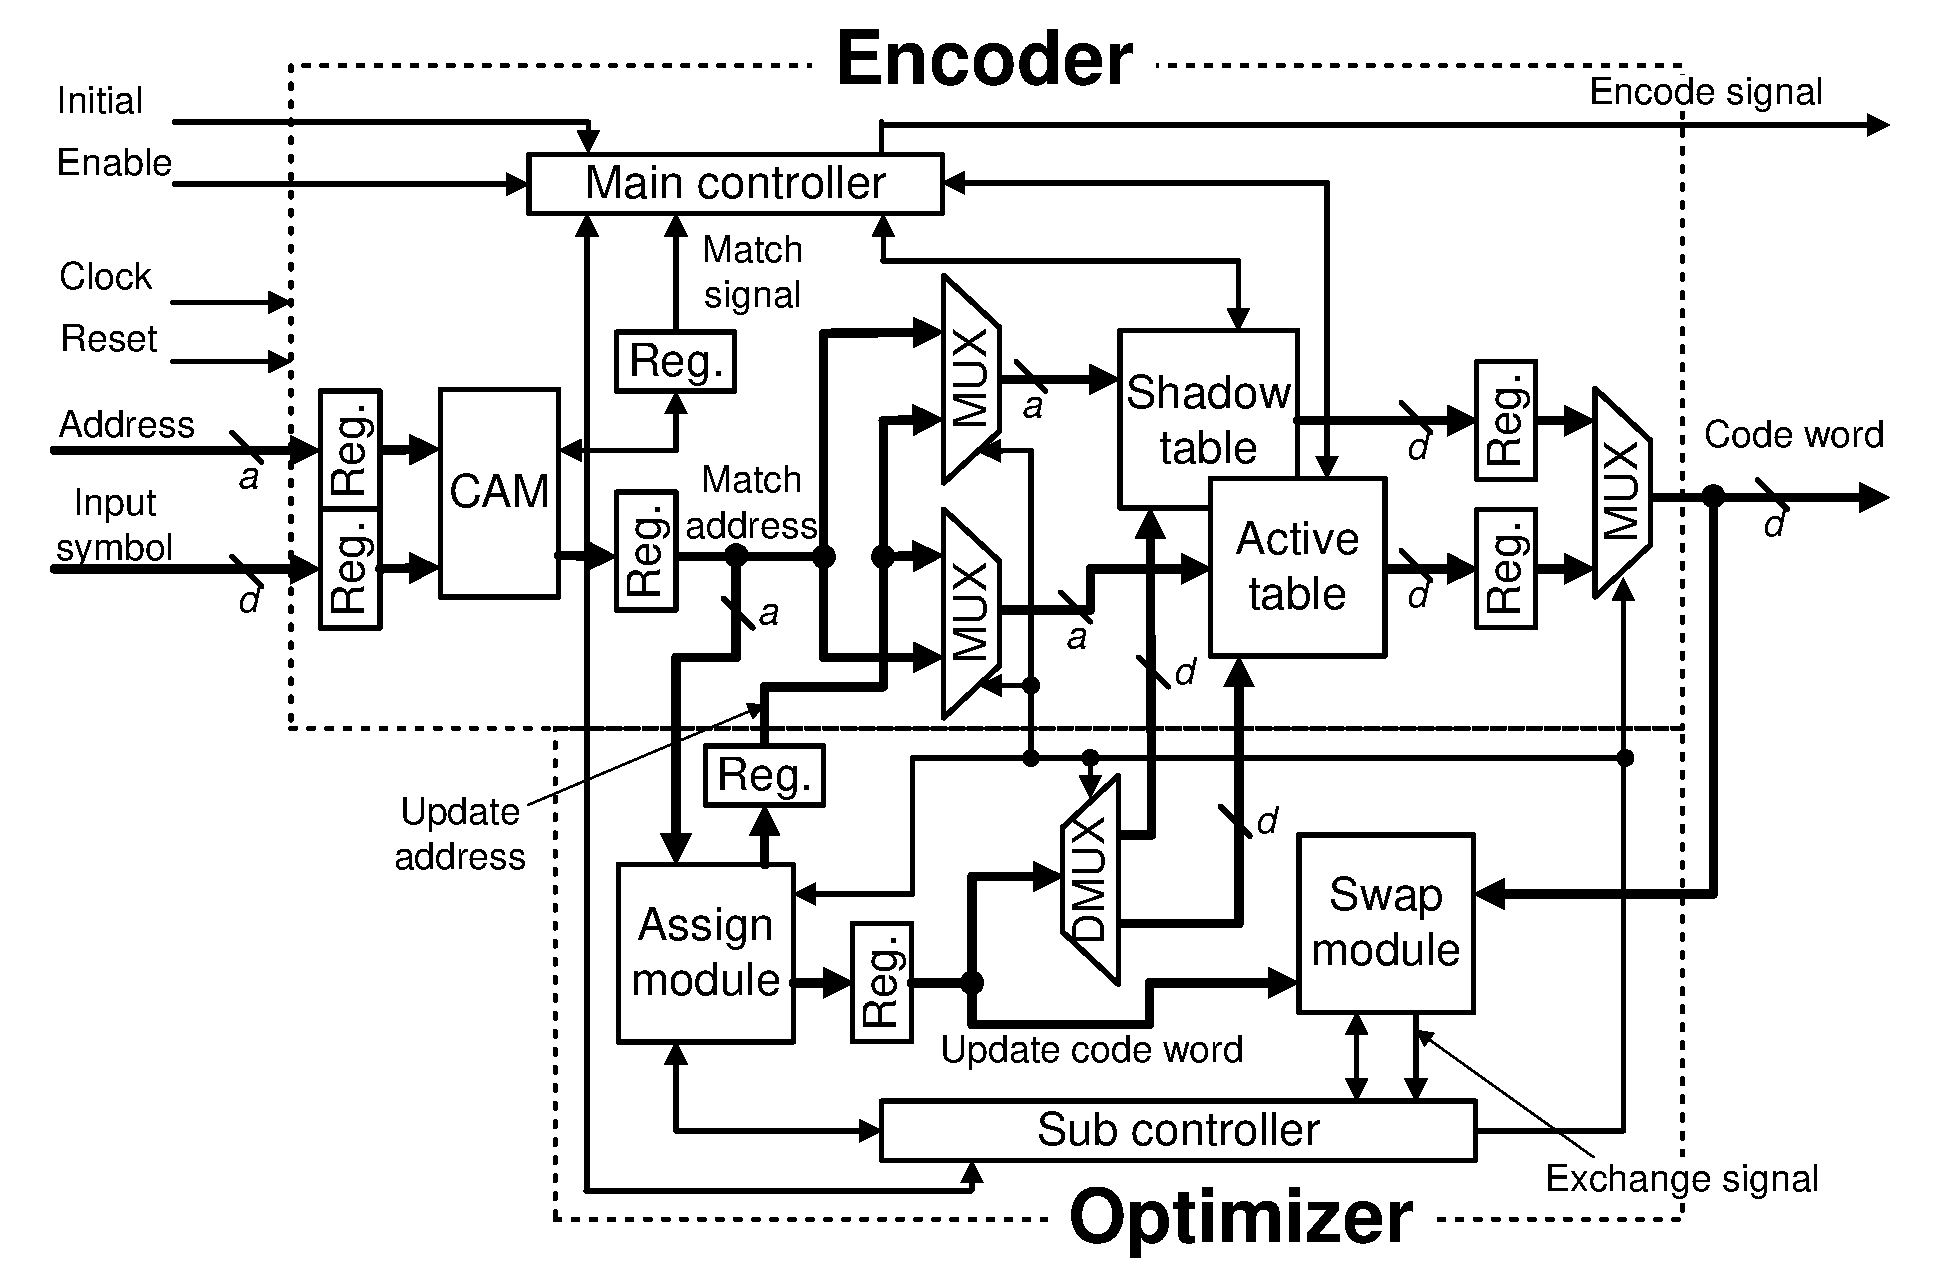
\includegraphics[width = 14cm, height = 14cm, keepaspectratio, clip]{./pics/block_dgrm.eps}
%		\caption{Detailed block diagram of the proposed architecture.}
		\caption{リアルタイム符号化テーブル最適化アーキテクチャブロック図.}
		\label{block_dgrm}
		\end{center}
	\end{figure}%
%\vspace{-3mm}
% figure*

\begin{itemize}
\item CAM (Content Addressable Memory)  $\times$  1
\item SRAM (Static Random Access Memory)  $\times$  2
\item マルチプレクサ (MUX: MUltipleXer)  $\times$  3
\item メインコントローラ (Main controller)  $\times$  1
\end{itemize}

内部のCAM及びSRAMは,ワード数$2^a$ (aはアドレス長),ワード長$d$-bitである.
また,2つのSRAMは,それぞれアクティブ符号化テーブル (以下,アクティブテーブルと呼ぶ)と,シャドウ符号化テーブル (以下,シャドウテーブルと呼ぶ)
を構成する.マルチプレクサは各種信号の切り替えに使用し,メインコントローラがこれらのモジュールを制御する.

オプティマイザブロックは,大きく分けて以下に示す4種類のモジュール及び複数個のレジスタから構成される.
\begin{itemize}
\item アサインモジュール (Assign module)  $\times$  1
\item スワップモジュール (Swap module)  $\times$  1
\item デマルチプレクサ (DMUX: DeMUltipleXer)  $\times$  1
\item サブコントローラ (Sub controller) $\times$  1
\end{itemize}

アサインモジュールと,スワップモジュールの働きについては,\ref{lbl_cp3_architecture}節にて詳述する.
デマルチプレクサは信号の振り分けを行い,サブコントローラはオプティマイザブロックの制御を担当する.


提案アーキテクチャは,エンコーダブロックとオプティマイザブロックが
並列に動作することによってリアルタイムに符号化テーブルを最適化した圧縮処理を実現する.その動作原理を,図 \ref{enc_pro}に示す.
図中に示すように,CAMには,入力される符号化前データの全パターンが格納されており,
アクティブテーブル及びシャドウテーブルには,ハフマン符号化テーブルが格納されている.
また,あらかじめCAMに格納されている全符号化前データと,SRAM内のテーブルに格納されているハフマン符号は,
符号変換に対応するデータ同士をアドレスで関連付けてある.
処理の流れは以下の通り.

\begin{enumerate}
\item 符号化前データがCAMに入力されると,CAM内部に格納しているパターンに対して,一致検索処理が1クロックサイクルで実行される.
\item CAMから一致した符号化前データのアドレスが出力され,アクティブテーブルの読み出しポートに入力される.
\item アクティブテーブルは,アドレスに基づき,入力された符号化前データに対応したハフマンコードを1クロックサイクルで出力する.
\item シャドウテーブルは,圧縮処理のバックグラウンドでデータの出現頻度にあわせてテーブルの内容が最適化されているため,
			圧縮効率が低下したならば即座に,アクティブテーブルとシャドウテーブルの役割を切り替える.これによって圧縮効率の向上を実現することが可能となる.
\end{enumerate}

提案アーキテクチャは,この一連のプロセスを,CAMに備えている検索データを格納するレジスタと,
SRAMに備えているアドレスレジスタを経由することで1クロックづつ符号化前データを移動させることができる.
そのためパイプライン処理を実現でき,連続して入力される符号化前データは,
1クロックサイクルで次々とハフマンコードに変換され出力される.
更に,エンコーダブロックは,入力される符号化前データの出現頻度にあわせ,符号化テーブルを選択することが可能である.
通常のハフマン符号化アーキテクチャは,既存のハフマン符号化テーブルを1つ備えているだけであり,符号化前データの
出現頻度が変化してもテーブルを選択することはできない.
提案アーキテクチャは,符号化処理と並行してシャドウテーブルのアップデートが行われており,
データの圧縮率があらかじめ定めてあるしきい値 (Threshold value)を下回った場合に,即座に符号化テーブルを切り替えることによって,
再び圧縮率を向上させることが可能となっている.
従来のハフマン符号化アーキテクチャは,符号化前データの出現頻度の変化に備えて,
複数のハフマン符号化テーブルを用意しているものもあるが\cite{matiwa95},
提案アーキテクチャは,アクティブテーブルとシャドウテーブル2つのみで様々な出現データに対応でき,かつ高い圧縮率を
実現することが可能となっている.


% figure*
	\begin{figure}[thb]
	\centering
		\begin{center}
			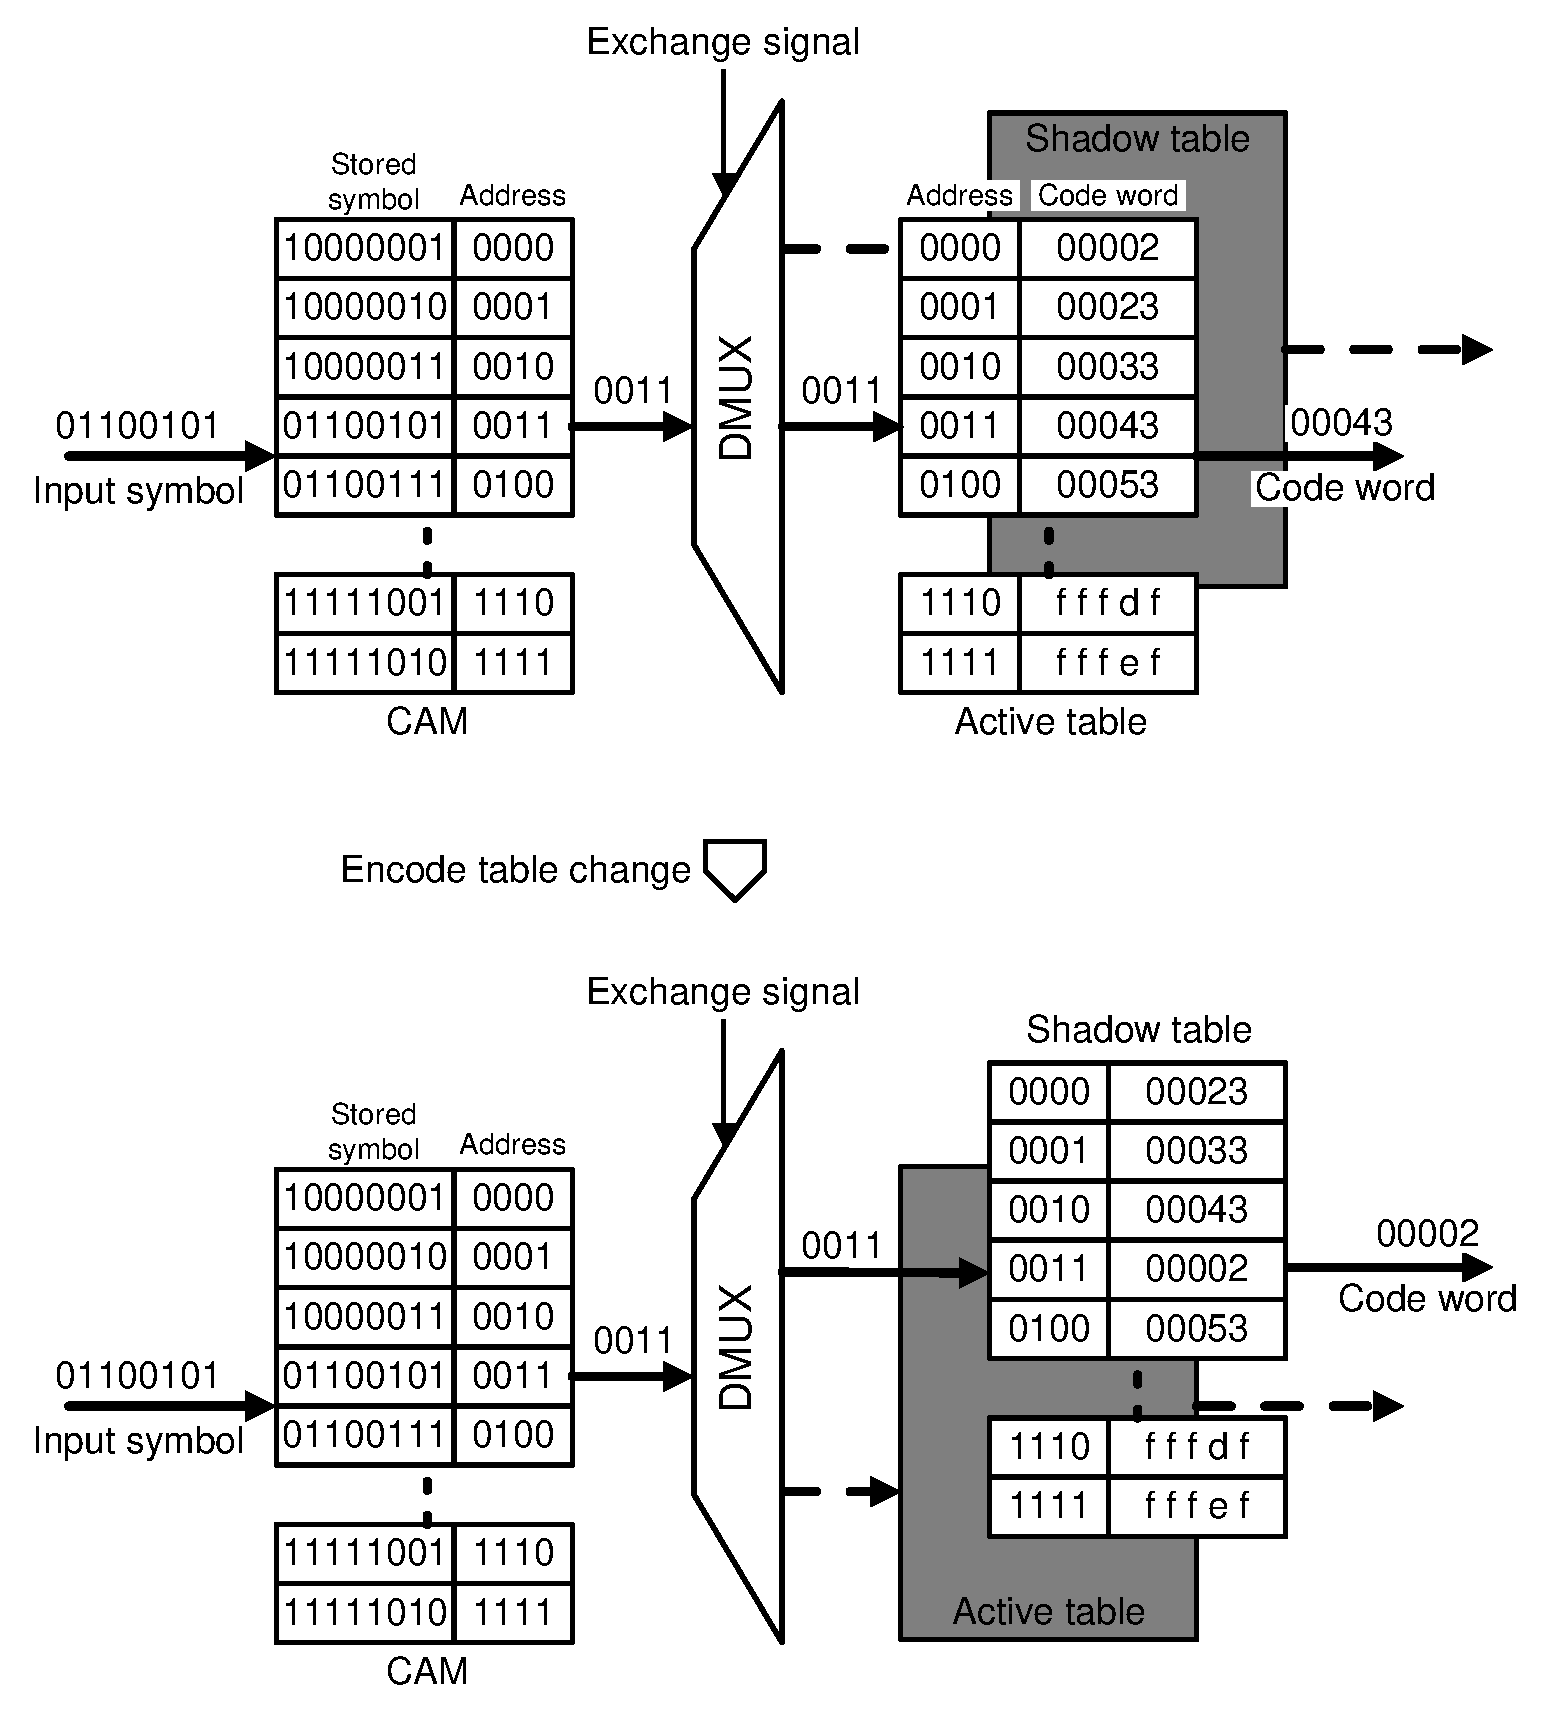
\includegraphics[width = 12cm, height = 12cm, keepaspectratio, clip]{./pics/enc_pro.eps}
		\caption{最適化された符号化テーブルを用いたリアルタイム圧縮処理動作原理.}
		\label{enc_pro}
		\end{center}
	\end{figure}%
%\vspace{-3mm}
% figure*

\subsection{リアルタイム符号化テーブル最適化の原理}
\label{lbl_cp3_real_opti_enc_pri}

提案アーキテクチャは,符号化テーブルをアクティブ用とアップデート用に分け,
符号化と並行してリアルタイムにマルチメディアデータの出現頻度を算出している.
そして,算出結果に基づき符号化テーブルをアップデートし,
データの圧縮状況にあわせてリアルタイムに符号化テーブルを切り替えることによって,
データの高圧縮の実現を可能としている.
この最適化は,図 \ref{block_dgrm}に示しているアサインモジュールとスワップモジュールによって実現される,
ハフマンテーブルの最適化及びアップデートのフローチャートを図 \ref{enc_flw}に示す.
図 \ref{enc_flw}の右側に示しているのが,オプティマイザブロックによるステップであり,
左側に示しているのが,エンコーダブロックによるステップである.
エンコーダブロックによるハフマン符号化に関しては,\ref{lbl_cp3_real_opti_enc}節で述べたとおりである.

% figure*
	\begin{figure}[thb]
	\centering
		\begin{center}
			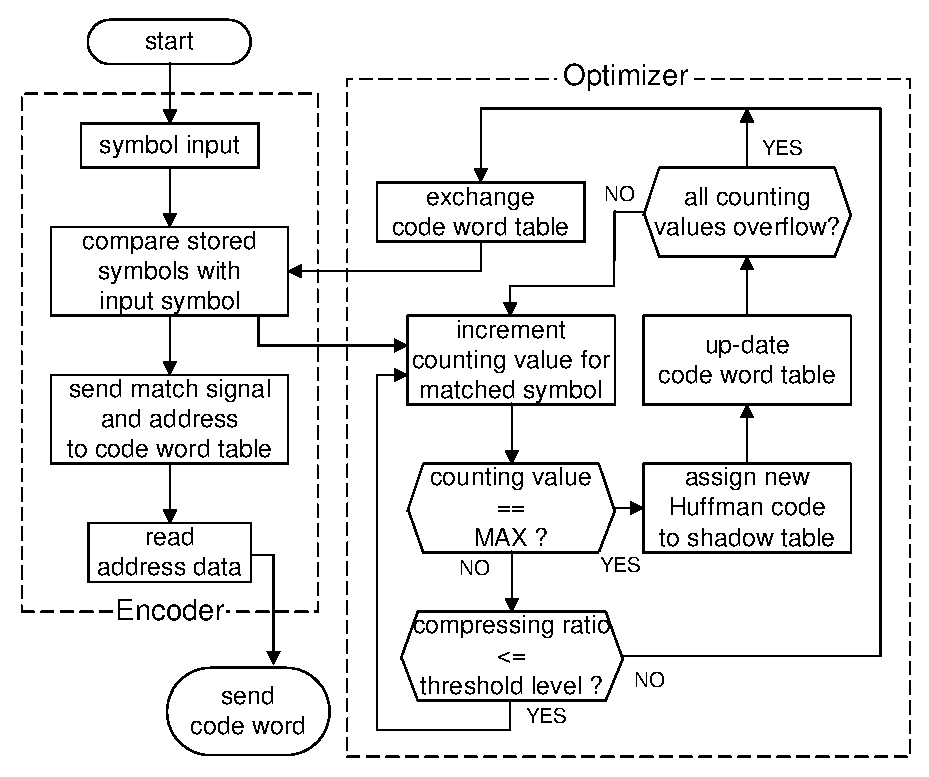
\includegraphics[width = 12cm, height = 12cm, keepaspectratio, clip]{./pics/enc_flw.eps}
%		\caption{Processing flow diagram of the proposed architecture.}
		\caption{ハフマンテーブルの最適化及びアップデートのフローチャート.}
		\label{enc_flw}
		\end{center}
	\end{figure}%
%\vspace{-3mm}
% figure*

オプティマイザブロックによるハフマンテーブルの最適化及びアップデートは符号化と並行して行われ,エンコーダブロックによる
パイプライン処理を妨げることは無い.
提案アーキテクチャに入力された符号化前データは,CAMで一致検索処理されアドレスに変換された後に,アクティブテーブルへ送信されるが,
同時にアサインモジュールにも送信される.
アサインモジュールには,CAMに格納されている全符号化前データパターンと同数個のカウンタが用意されており,
CAMの一致検索結果に従って,該当するカウンタがインクリメントされる.

アサインモジュールは,1回の符号化毎にカウンタのインクリメントが終了した後,該当したカウンタの値がオーバフロー
していないか確認する.ここでオーバフローを確認した場合には,その直前に入力された符号化前データの出現頻度が
大きいことを意味するため,現在変換に利用されているハフマンコードより,短いビット長のアップデート用ハフマンコードを
シャドウテーブルへ送信する.このアップデート用ハフマンコードはCAMから出力された一致アドレスが示すデータへ上書きされることとなる.
続いてアサインモジュールでは,内部に格納しているカウンタが全てオーバフローしているか否かを確認し,
全てのカウンタのオーバフローが確認されたならば,サブコントローラに確認信号を送信する.
その後,サブコントローラからテーブル切り替え信号 (Exchange signal)がスワップモジュールに送信され,アクティブテーブルとシャドウテーブルの
役割を切り替える信号がスワップモジュールからサブコントローラを介して送信されることとなる.

CAMによる一致検索処理に該当したカウンタが,オーバフローしていなかった場合は,ハフマンコードのアップデート
プロセスは省略されるものの,スワップモジュール内であらかじめ設定してあるしきい値と,現在の圧縮率を比較し,しきい値を
上回った場合には,アクティブテーブルとシャドウテーブルの役割を切り替える信号がスワップモジュールから送信される.

以上のプロセスによって,出現頻度の高い符号化前データには,よりビット長の短いハフマンコードが割り当てられ,
データの圧縮率が低下した場合には,新しく構築したハフマンテーブルが適用される.
従って,提案アーキテクチャは,常に画像等の出現データの特徴にあわせて,リアルタイムに高い圧縮率を維持することが可能となる.



%/**********************************************************************/
%		ハードウェアアーキテクチャを解説する章
%/**********************************************************************/

\subsection{アーキテクチャ}
\label{lbl_cp3_architecture}

この節では,提案アーキテクチャの符号化テーブルアップデート,及び切り替えの役割を担う,
オプティマイザブロックのアーキテクチャを中心に述べる.

\subsubsection{アサインモジュール}
\label{lbl_cp3_asgn_mdl}

入力される符号化前データの出現頻度に基づいたシャドウテーブルの最適化は,
主としてアサインモジュールによって処理される.
図 \ref{asgn_mod}に,アサインモジュール内部のブロック図を示す.
アサインモジュールは,大きく分けて以下に示す9種類のユニットが動作して
符号化テーブルのアップデート処理を実行する.

% figure*
	\begin{figure}[thb]
	\centering
		\begin{center}
			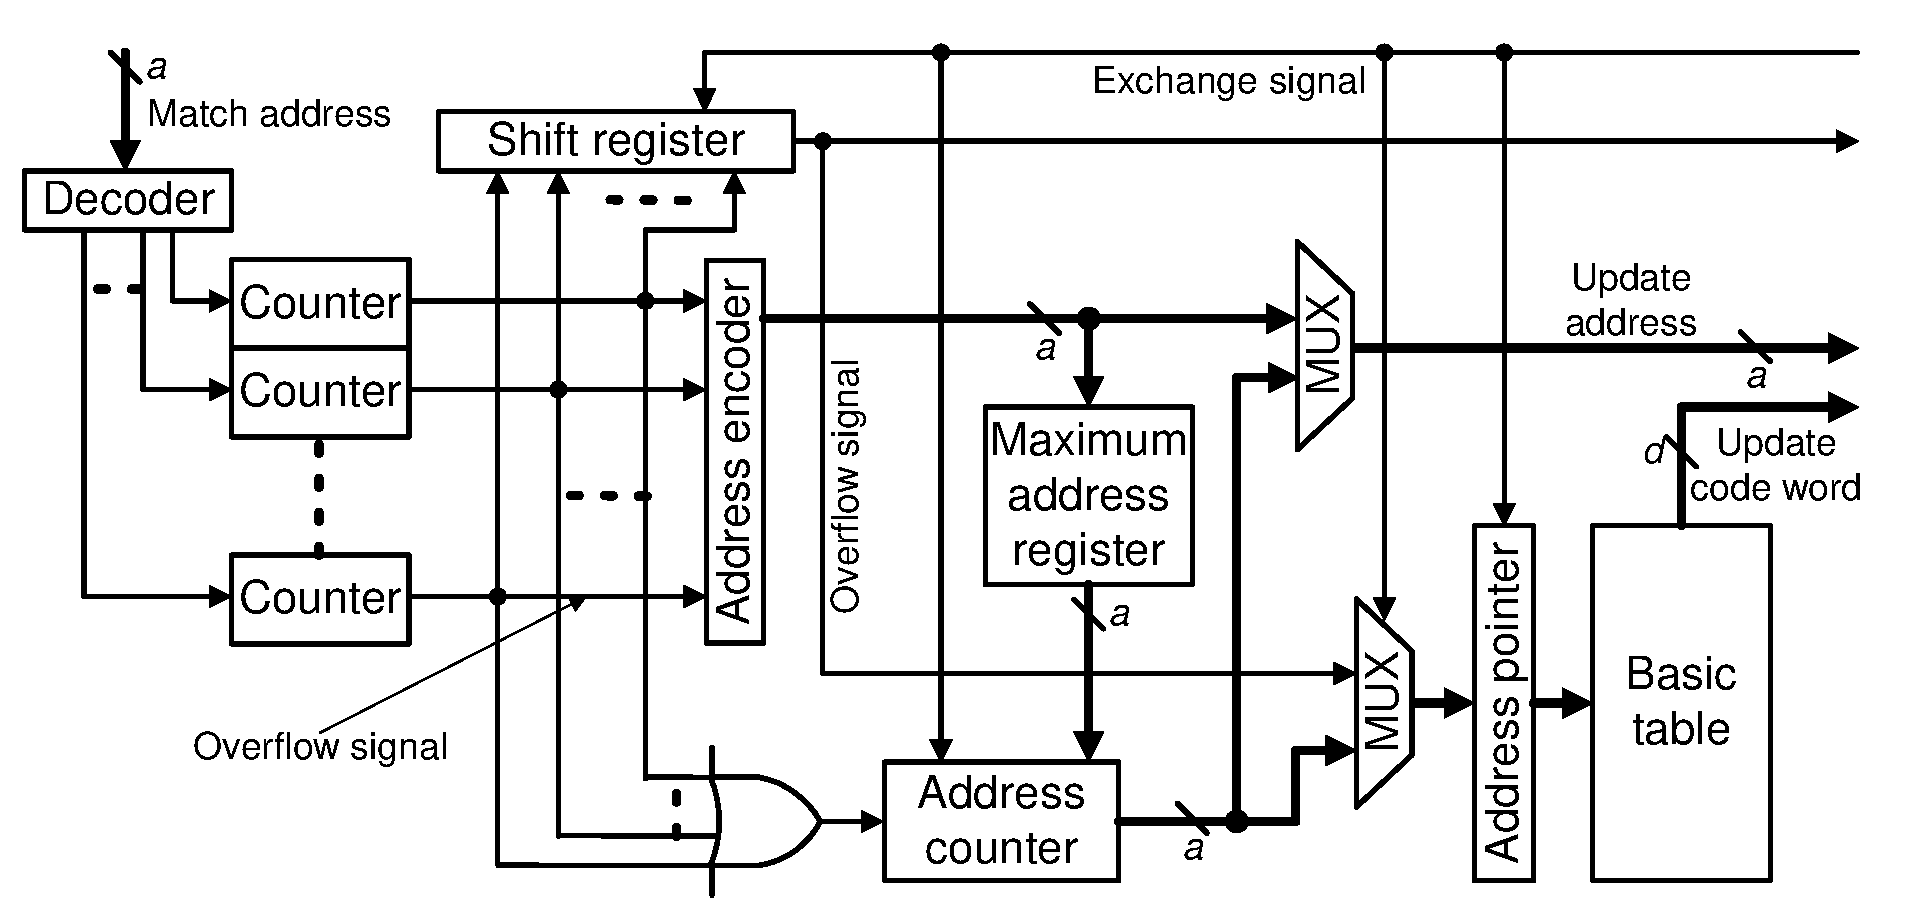
\includegraphics[width = 14cm, height = 14cm, keepaspectratio, clip]{./pics/asgn_mod.eps}
%		\caption{Block diagram of the assign module.}
		\caption{アサインモジュールブロック図.}
		\label{asgn_mod}
		\end{center}
	\end{figure}%
%\vspace{-3mm}
% figure*

\begin{itemize}
\item カウンタ (Counter)  $\times$  $2^a$ 
\item デコーダ (Decoder)  $\times$  1
\item アドレスエンコーダ (Address encoder)  $\times$  1
\item アドレスカウンタ (Address counter) $\times$  1
\item アドレスポインタ (Address pointer)  $\times$  1 
\item ベーシックハフマン符号化テーブル (Basic table)  $\times$  1
\item シフトレジスタ (Shift register)  $\times$  1
\item 最大アドレス値記憶用レジスタ (Maximum address register) $\times$  1
\item マルチプレクサ (MUX: MUltipleXer) $\times$  2
\end{itemize}

エンコーダブロックに内蔵されているCAMに,符号化前データが入力された後,一致アドレスはアサインモジュールに
入力される.
一致アドレスはデコーダを経由するため,$2^a$個あるカウンタのうち1つが選択され,その値がインクリメントされる.
この際,提案アーキテクチャを適用するアプリケーションによって,カウンタの最大値をあらかじめ決定しておく.
カウンタがオーバフローを起こした場合,オーバフローシグナル (Overflow signal)は,
アドレスエンコーダ (Address encoder)を経由してアドレス値に変換され,シャドウテーブルを更新するためのアップデートアドレス (Update address)として出力される.
それと同時に,オーバフローシグナルをOR演算した結果が,アドレスカウンタに入力されベーシックハフマン
符号化テーブル (以下ベーシックテーブルと呼ぶ)用の,アドレスが生成される.
シャドウテーブルを最適化するための,アップデートハフマンコード (Update code word)は,ビット長の短いものから
べーシックテーブルに降順で格納されているため,カウンタがオーバフローした順に,先に生成されたアップデートアドレス
に基づき,シャドウテーブルへアップデートハフマンコードが送られることとなる.
これらのカウンタ及びアドレスカウンタの値は,スワップモジュールによってアクティブテーブルとシャドウテーブルが切り替えられた後,
リセットされる.提案アーキテクチャは,この切り替え処理を2つの条件,
圧縮率があらかじめ設定されたしきい値を上回った場合,もしくは全カウンタがオーバフローした場合
に行う.

次にアサインモジュールに内蔵されている各ユニットの働きと共に,シャドウテーブルのアップデート手順を,図 \ref{asgn_pro}にて述べる.
処理開始時には,アクティブテーブル,シャドウテーブル,及びベーシックテーブルに格納されているデータは同一である.
カウンタのオーバフロー時に,アサインモジュールから出力されるアップデートハフマンコードは,
シャドウテーブルの別のアドレスに格納されている.そのため,アップデートハフマンコードを書き込む前に,
そのアドレスに書き込まれているハフマンコードは,
シャドウテーブル内の別のアドレスへ移さなければならない.
しかしながら,この入れ替え処理には少なくとも数クロックサイクル程度必要とするため,
エンコーダブロックのパイプライン処理の妨げとなる.
この問題を解決するために,提案アーキテクチャはシャドウテーブルのアップデートプロセスを,
オーバーライティングフェーズ (Over-writing phase),及びオーダーライティングフェーズ (Order-writing phase)
に分けて行うこととした.

オーバーライティングフェーズでは,シャドウテーブルのデータの整合性を気にすることなく,オーバフローした
カウンタに基づいて,次々にアップデートハフマンコードを上書きしていく.

図 \ref{asgn_pro}の例に示すように,アップデートハフマンコード,``00002"及び``00023"は,同一のデータがテーブル内に
存在するのに関わらず上書きされているのが分かる.
アップデートハフマンコード,``00002"は,2 bitのデータ量であり,上書き前のデータである``001e5"と比較して3 bitのデータ量削減となる.
この例の場合,3回のアップデートが行われたため,合計20 ($ = $3$ + $13$ + $4) bitのデータ量削減となる.
また,カウンタから出力されるオーバフローシグナルは,信号線が接続されているシフトレジスタの各ビットへ書き込まれ,
最大アドレス値記憶用レジスタは,アドレス``0010"から``1110"に更新される.
以上の処理をアサインモジュールは,カウンタ全てがオーバフローするか,圧縮率がしきい値を
上回るまで実行する.

オーダーライティングフェーズは,オーバーライティングフェーズで生じた,シャドウテーブル内のデータの不整合を
修正する処理である.
オーバーライティングフェーズ終了時には,異なる符号化前データでも,同一のハフマンコードが出力される状態となっている.
そのため,降順で読み出されたベーシックテーブルのハフマンコードの残りを,最大アドレス記憶用レジスタが示すアドレスまで
シャドウテーブルに書き込まなければならない.
オーバーライティングフェーズが終了したならば,図 \ref{asgn_mod}に示す,アドレスポインタは最後のアップデートアドレスの
位置で停止する.
その後アドレスカウンタは,再び0からカウントを開始し,シャドウテーブルにアドレスを送信する.
この時,シフトレジスタはこれまで保存していたオーバフローの履歴を逐次的に出力する.
この信号は,シャドウテーブルへはデータ書込みのイネーブル信号として,ベーシックテーブルへは
アドレスポインタをオフセットとして残りのアップデートハフマンコードを読み出すアドレスとして利用される.

図 \ref{asgn_pro}の例では,シャドウテーブルには,アドレス``0000"に,``001e5"の続きのハフマンコードである``00fe8"が
書き込まれる.続いてアドレス``0001"には,ハフマンコード``00fa9"が書き込まれる.
この処理を最大アドレス記憶用レジスタが保存しているアドレス``1110"まで繰り返す.
その結果,ハフマンコードが重複すること無く,シャドウテーブルは,入力される符号化前データの出現頻度にあわせてアップデートされる.

以上述べた,オーバーライティングフェーズとオーダーライティングフェーズは,符号化のパイプライン処理を停止することなく
実行されるため,提案アーキテクチャは高速にハフマン符号化を実行しながら,ハフマンテーブルの切り替えを実現できる.


% figure*
	\begin{figure*}[hbt]
	\centering
		\begin{center}
			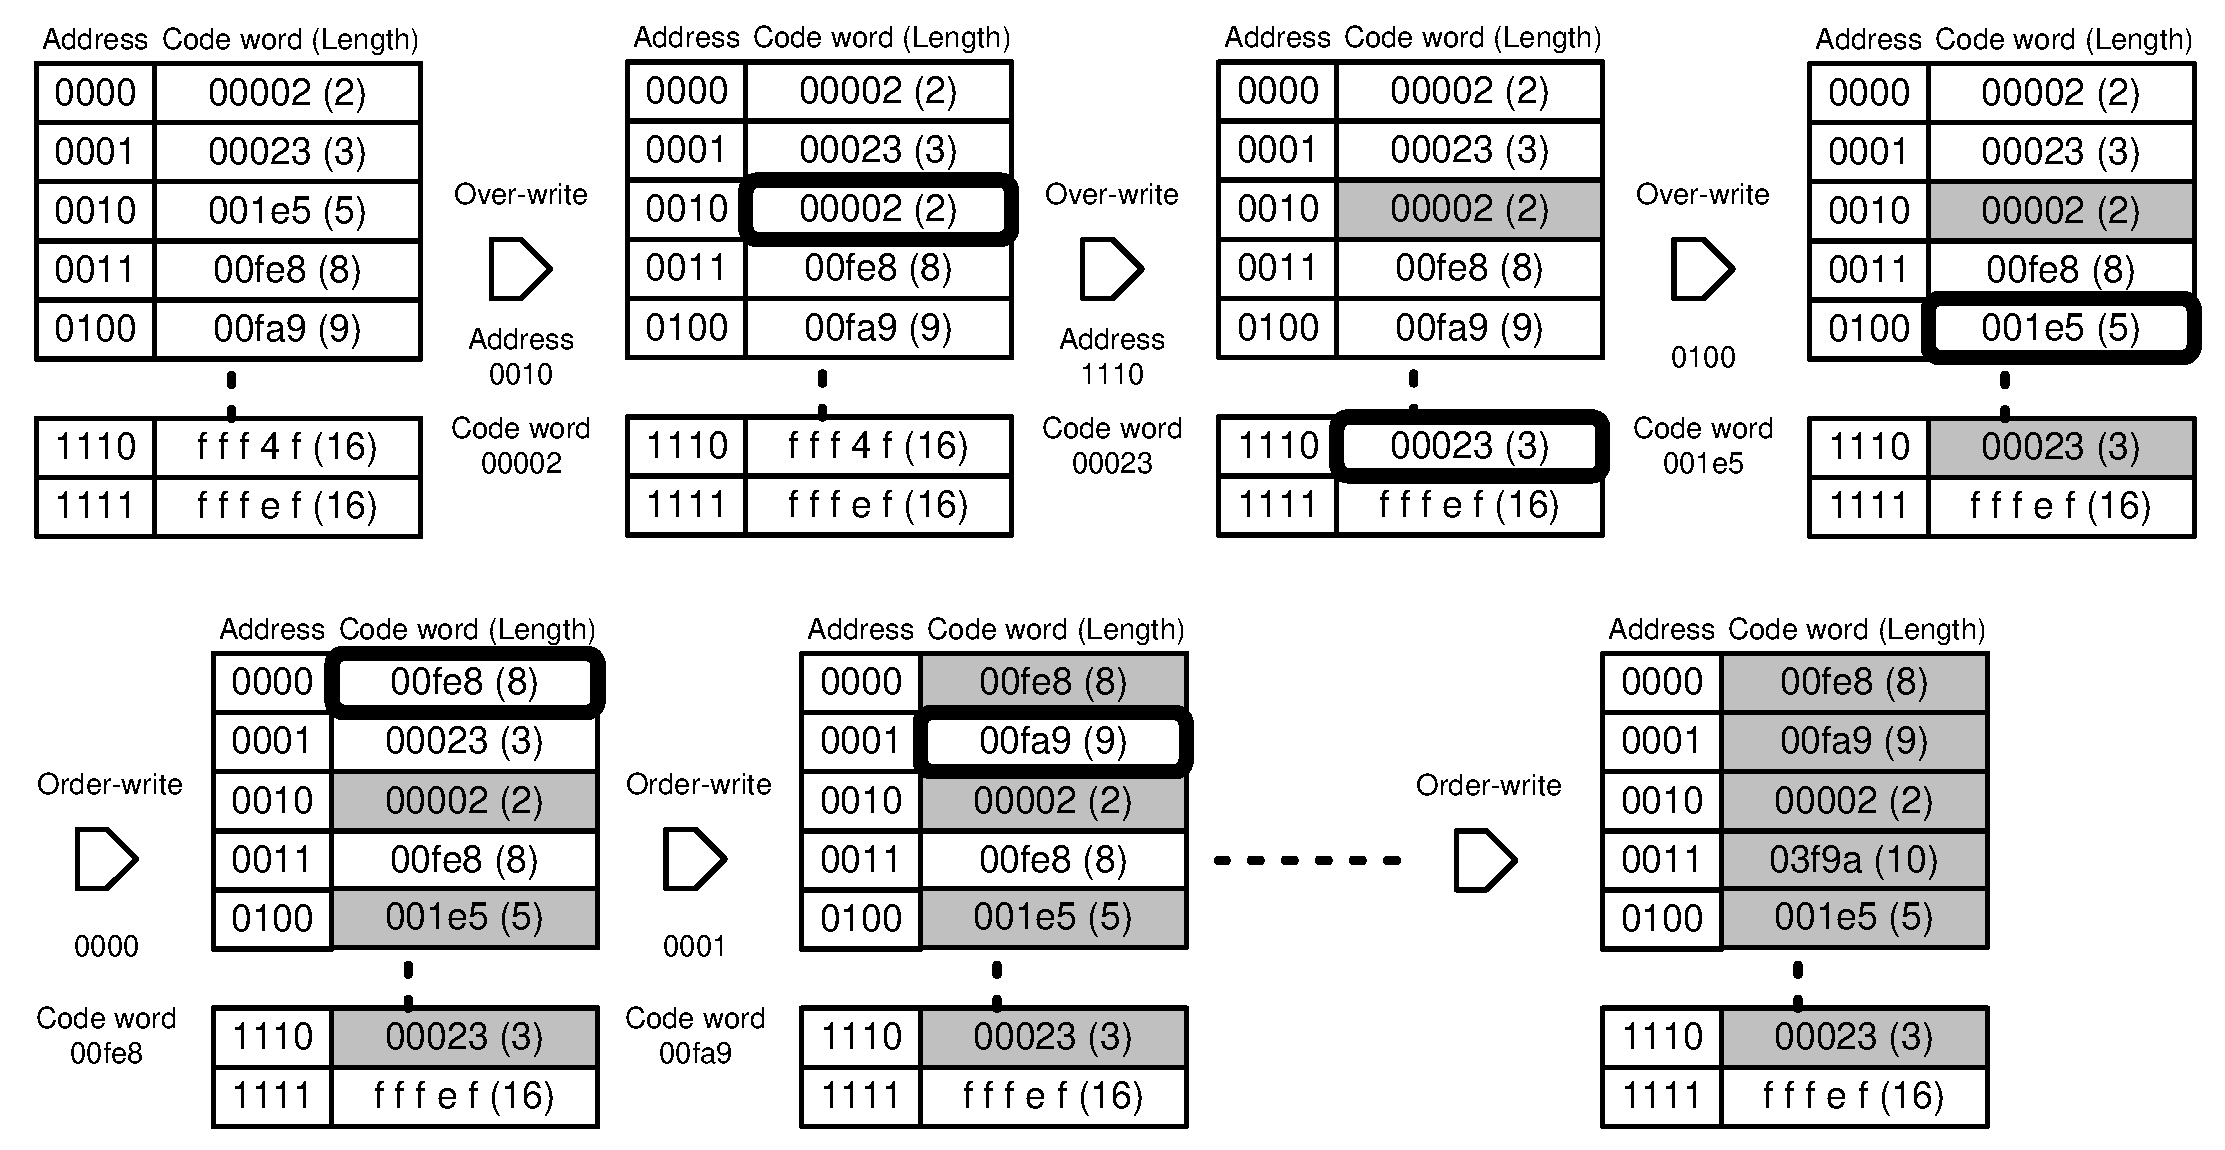
\includegraphics[width = 14cm, height = 14cm, keepaspectratio, clip]{./pics/asgn_pro.eps}
%		\caption{Procedure of optimizing the shadow code word table.}
		\caption{シャドウテーブルのアップデート処理手順.}
		\label{asgn_pro}
		\end{center}
	\end{figure*}%
%\vspace{-3mm}
% figure*

\subsubsection{スワップモジュール}
\label{lbl_cp3_swp_mdl}

スワップモジュールは,符号化前データの圧縮状況を監視し,アクティブテーブルとシャドウテーブルの切り替えを
実行するモジュールである.
図 \ref{swap_mod}に,ブロック図を示す.
スワップモジュールは,大きく分けて以下に示す4種類のユニットから構成される.

% figure*
	\begin{figure}[tbh]
	\centering
		\begin{center}
			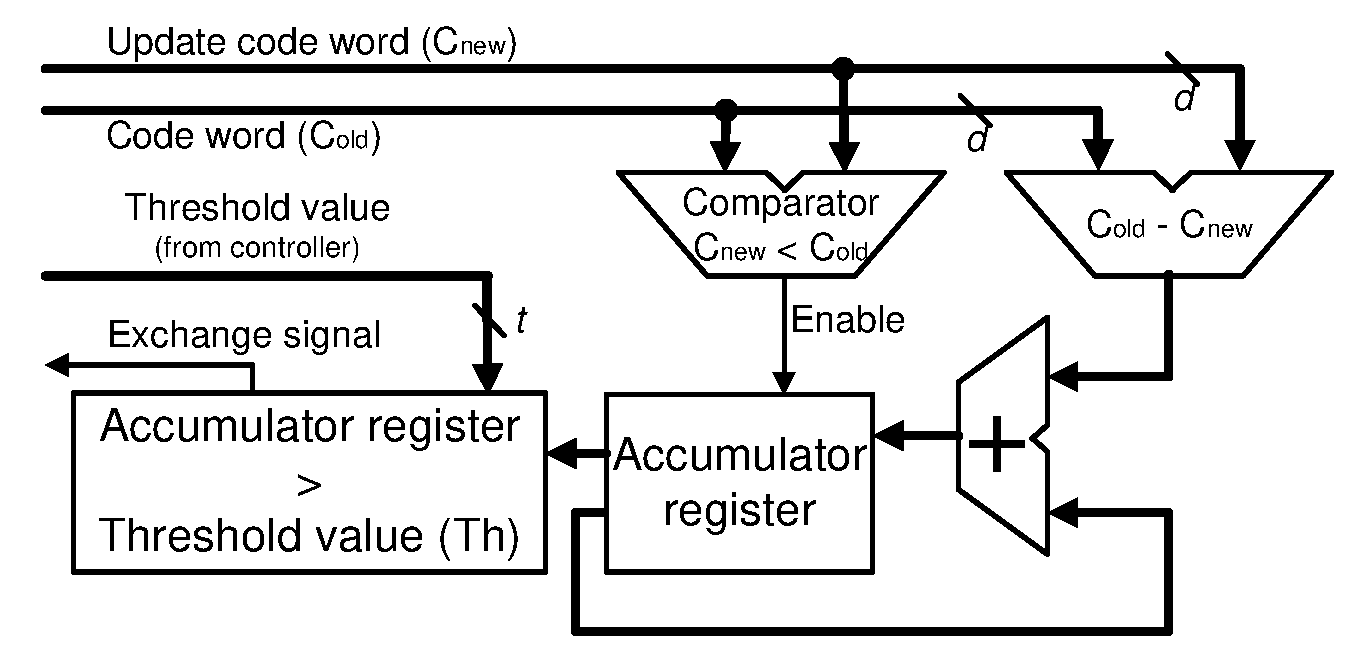
\includegraphics[width = 12cm, height = 12cm, keepaspectratio, clip]{./pics/swap_mod.eps}
		\caption{スワップモジュールブロック図.}
		\label{swap_mod}
		\end{center}
	\end{figure}%
%\vspace{-3mm}
% figure*

\begin{itemize}
\item アキュムレータレジスタ (Accumulator register)  $\times$  $2^a$ 
\item 加算器 (Adder)  $\times$  1
\item 減算器 (Subtractor)  $\times$  1
\item 比較器 (Comparator) $\times$  2
\end{itemize}

エンコーダブロックにてハフマンコード(Code word: C$_{old}$)が出力され,アサインモジュールがアップデート
ハフマンコード (Update code word: C$_{new}$)を生成した場合,
スワップモジュールは,これらデータの減算処理 (C$_{new}$ $-$ C$_{old}$)を行う,
また,比較器では,データの大小比較 (C$_{new}$ $<$ C$_{old}$)を行い,アップデートハフマンコードが
出力されたハフマンコードより小さい場合,減算結果が加算器を介してアキュムレータレジスタへ保存される.
このアキュムレータレジスタに保存される値は,これまでアップデートされたハフマンコードが,
どの程度ビット長を削減しているかの指標として利用できる.
よって,この指標があらかじめユーザによって指定されるしきい値を超えた場合,現在の
アクティブテーブルは入力される符号化前データに適応していないことがわかる.
その結果,スワップモジュールは直ちにアクティブテーブルとシャドウテーブルの切り替え信号 (Exchange signal)を
生成するため,提案アーキテクチャはどのようなパターンの符号化前データが入力されても,圧縮効率の向上を実現することが可能となる.
